\documentclass[border=10pt]{standalone}
\usepackage{tikz} 

\begin{document}
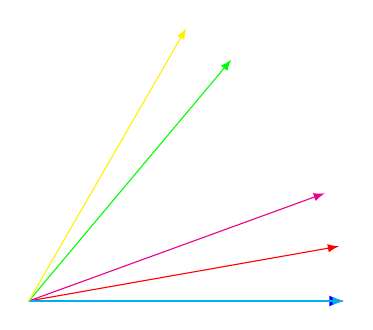
\begin{tikzpicture}

\draw[-latex, red, rotate around={10:(0,0)}] (0,0) -- (4,0);

\draw[-latex, magenta, rotate around={20:(0,0)}] (0,0) -- (0:4);

% behaviour not as expected
\coordinate (last1) at (4,0);
\draw[-latex, blue, thick, rotate around={30:(0,0)}] (0,0) -- (last1);

% behaviour not as expected
\coordinate (last2) at (0:4);
\draw[-latex, cyan, rotate around={40:(0,0)}] (0,0) -- (last2);


\coordinate (last3) at (4,0);
\draw[-latex, green] (0,0) -- ([rotate=50]last3);

\coordinate (last4) at (0:4);
\draw[-latex, yellow] (0,0) -- ([rotate=60]last4);

\end{tikzpicture}
\end{document}